We compute the upper limits using the shape of the LR to maximize the analysis sensitivity as described in 
Section~\ref{sec:results}. The expected upper limit at 95\%C.L correspoinding to 1~$\ifb$ 
as a function of $m_H$ using the LR are shown in Figure~\ref{fig:me_expected_1fb} 
comparing the corresponding results using the BDT output. 
In the calculation, we apply overal data-to-simualtion scale factors to the yields predictd by simulation.  
%The scale factor for the SM Higgs is 1.13, 1.9 for the $\ttbar+tW$ and $\Wjets$, and 2.6 $\dyll+WZ+ZZ$. 
The sensitivity performance of the matrix element method is consistent with the BDT based approach.
% with a slightly larger exclusion region. 
The results for each mass points are tabulated in Table~\ref{tab:me_expected_1fb}. 

%%%%%%%%%%%%%%%%%%%%%%%%%%%%%%
\begin{figure}[!hbtp]
\centering
\subfigure[]{
\centering
\label{subfig:me_exp_1fb}
%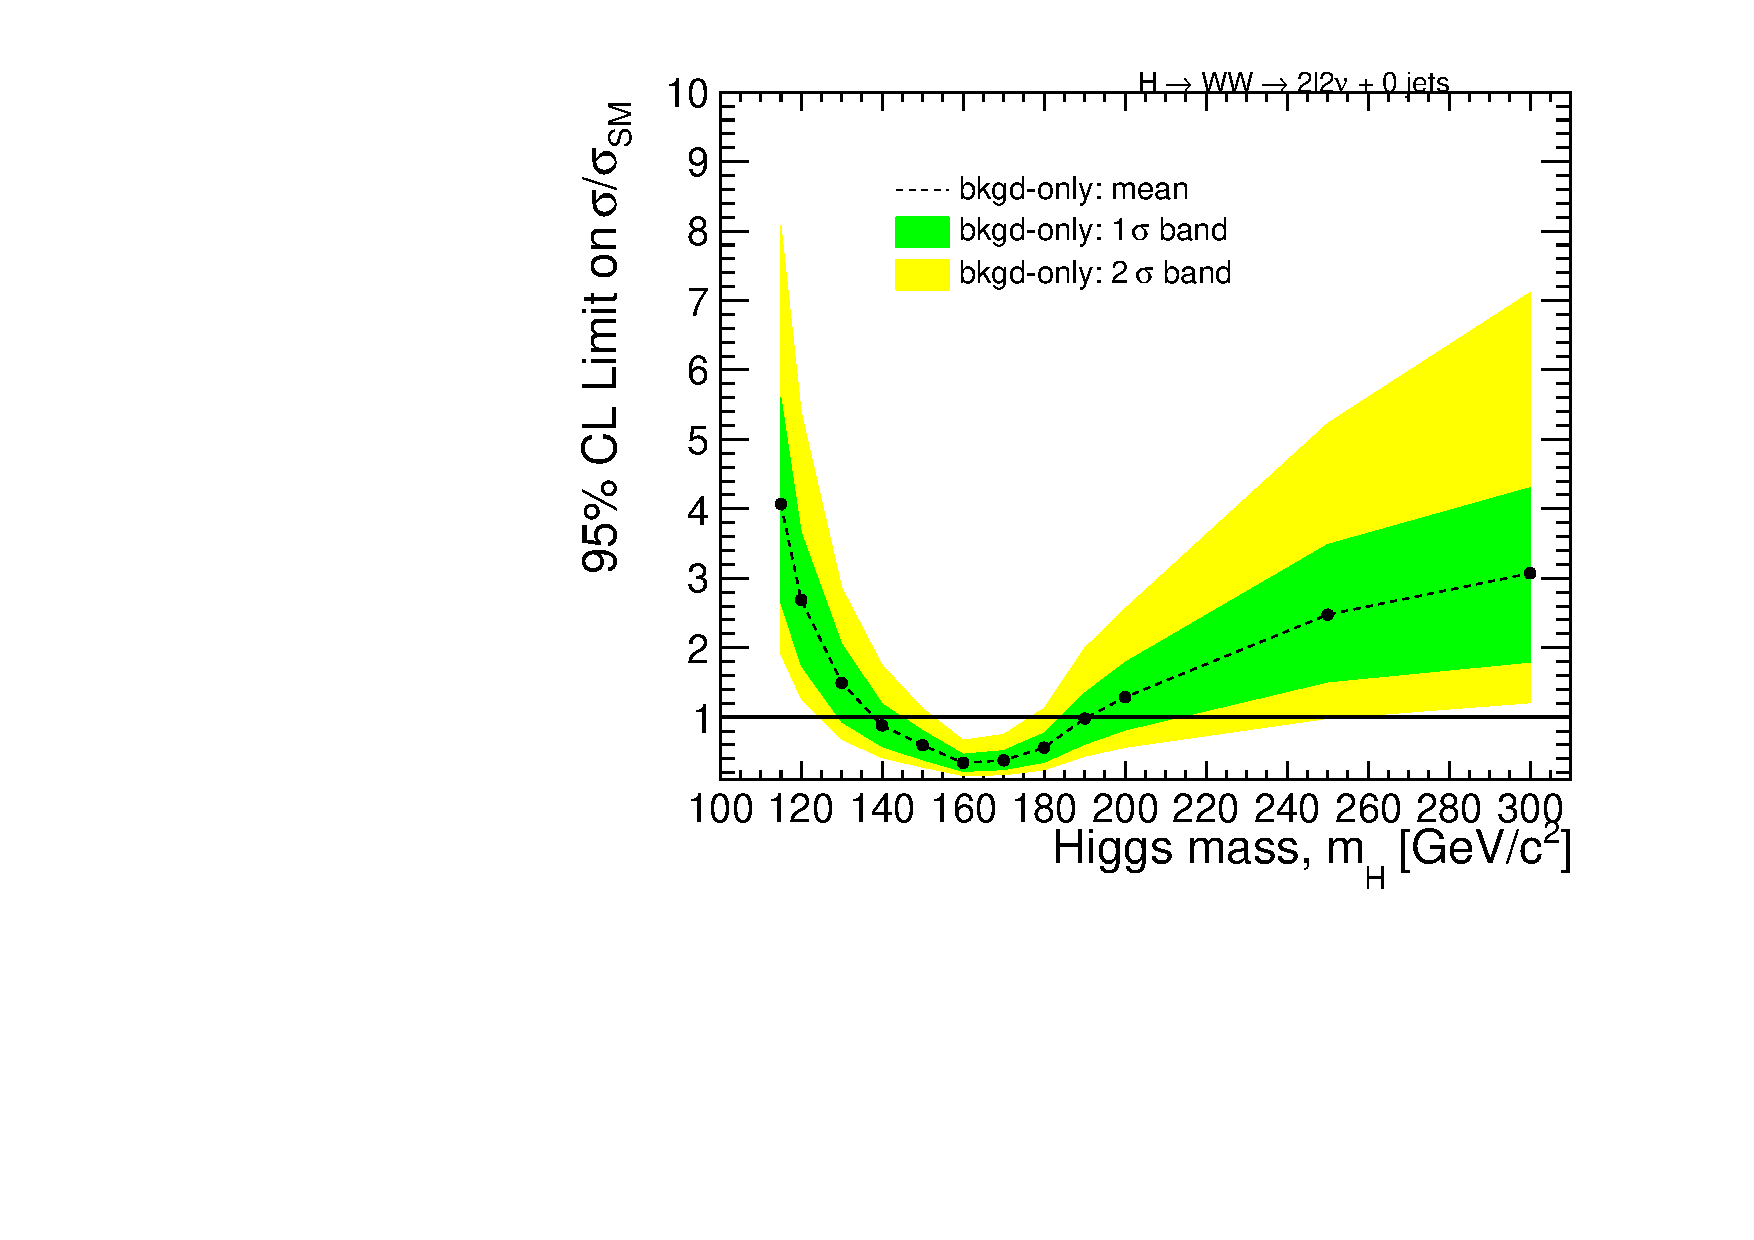
\includegraphics[width=.45\textwidth]{figures/limits_0j_1000pb_ME_shape.pdf}
}
\subfigure[]{
\centering
\label{subfig:bdt_exp_1fb}
%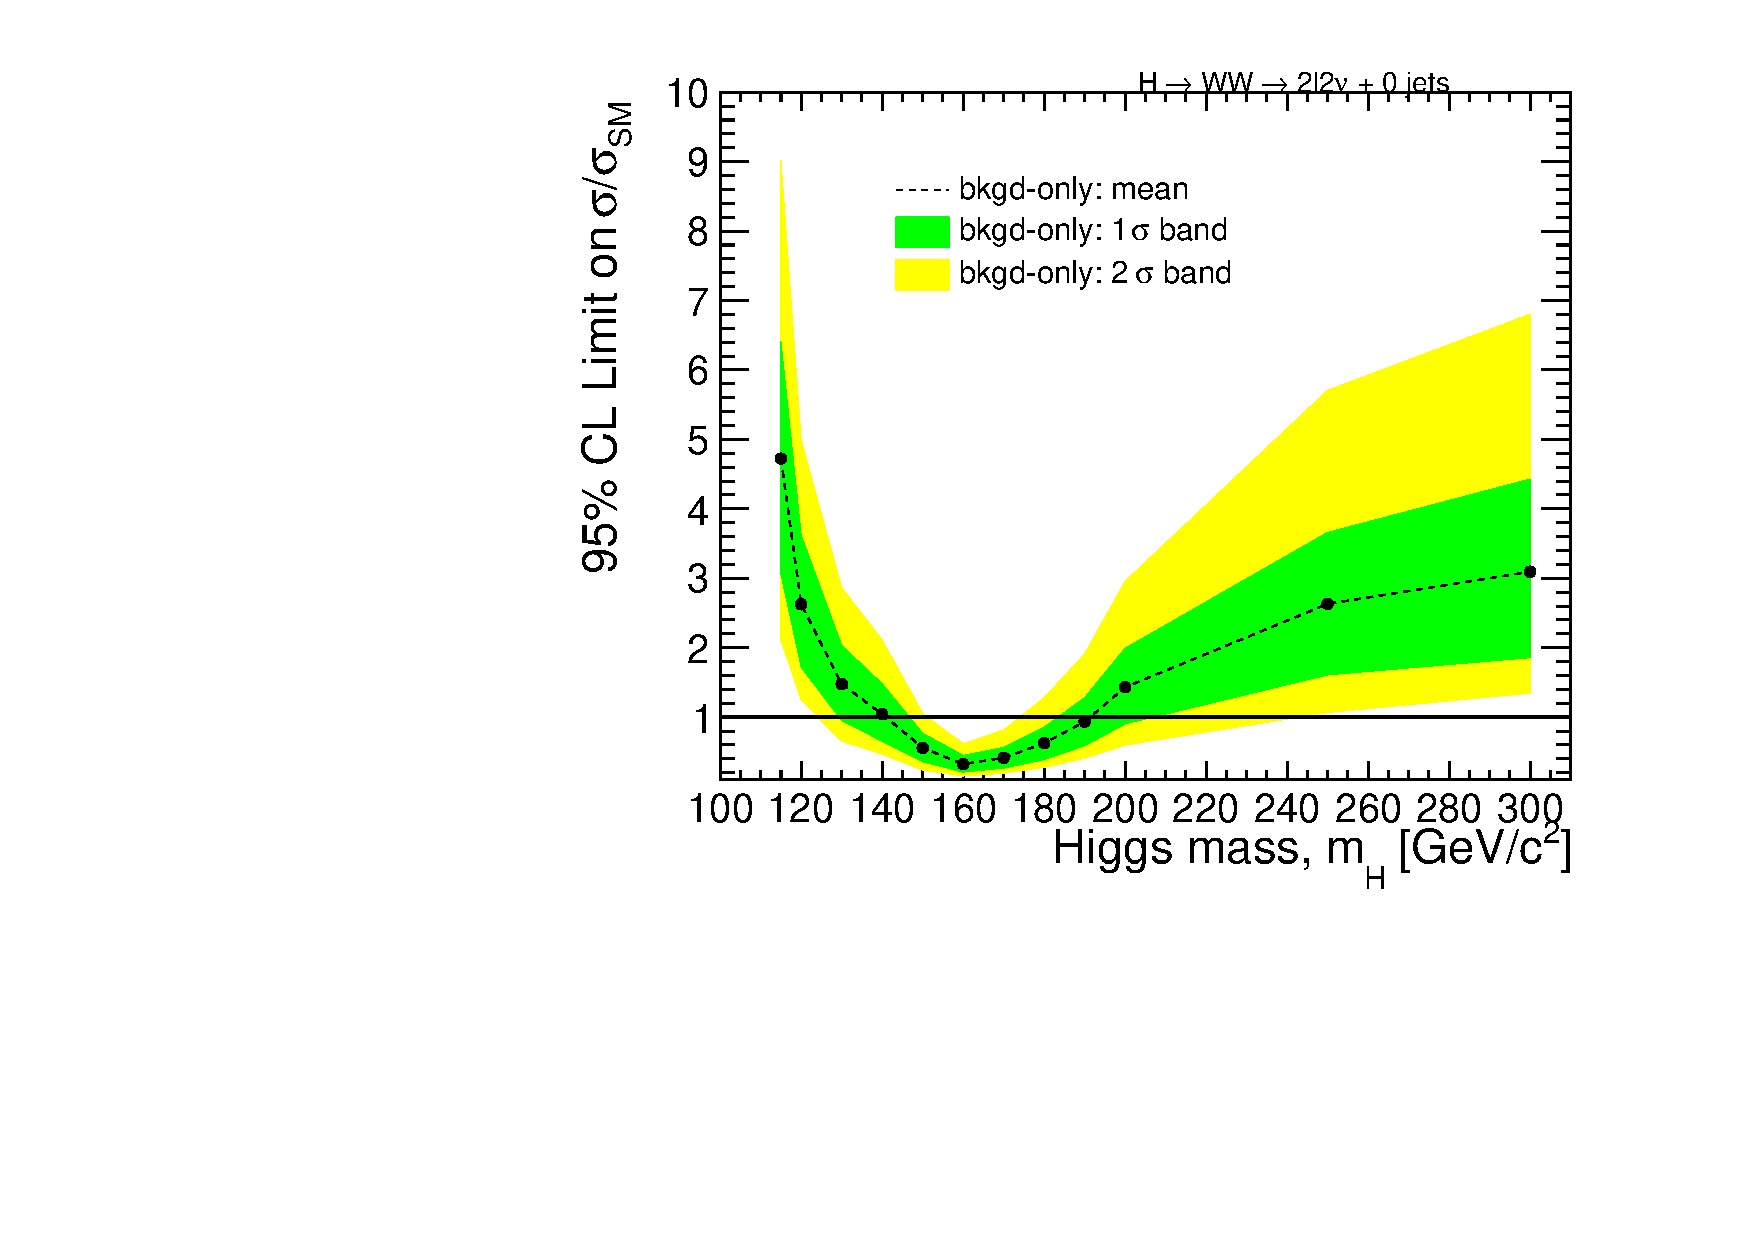
\includegraphics[width=.45\textwidth]{figures/limits_0j_1000pb_BDT_shape.pdf}} \\
}
\caption{ 
Multivariate shape analysis expected upper limits at 95\% C.L. for 1~$\ifb$ data using the 
matrix elemement output \subref{subfig:me_exp_1fb} and BDT output \subref{subfig:bdt_exp_1fb}. } 
\label{fig:me_expected_1fb}
\end{figure}
%%%%%%%%%%%%%%%%%%%%%%%%%%%%%%

%%%%%%%%%%%%%%%%%%%%%%%%%%%%%%
\begin{table}
\begin{center}
\begin{tabular}{c c c c c c c}
\hline\hline
 $m_H$ (GeV) & $-2\sigma$ & $-\sigma$ & median & $+1\sigma$ & $+2\sigma$ \\
\hline
\multicolumn{6}{c} {Matrix Element Method} \\
\hline
 115 & 1.66 & 2.23 &  3.17 &  4.48 &  6.23 \\
 120 & 1.02 & 1.40 &  2.03 &  2.88 &  4.08 \\
 130 & 0.56 & 0.78 &  1.11 &  1.63 &  2.32 \\
 140 & 0.37 & 0.51 &  0.74 &  1.05 &  1.49 \\
 150 & 0.24 & 0.36 &  0.50 &  0.72 &  1.02 \\
 160 & 0.15 & 0.21 &  0.29 &  0.42 &  0.63 \\
 170 & 0.17 & 0.23 &  0.33 &  0.47 &  0.68 \\
 180 & 0.22 & 0.32 &  0.46 &  0.69 &  0.97 \\
 190 & 0.39 & 0.54 &  0.78 &  1.16 &  1.59 \\
 200 & 0.49 & 0.69 &  1.03 &  1.49 &  2.18 \\
 250 & 0.82 & 1.24 &  1.75 &  2.70 &  4.07 \\
 300 & 1.00 & 1.44 &  2.10 &  3.27 &  4.87 \\
\hline
\multicolumn{6}{c} {BDT Based} \\
\hline
 115 & 1.57 & 2.17 &  3.22 &  4.53 &  6.89 \\
 120 & 1.03 & 1.43 &  2.04 &  2.95 &  4.03 \\
 130 & 0.55 & 0.75 &  1.10 &  1.60 &  2.25 \\
 140 & 0.34 & 0.48 &  0.69 &  1.00 &  1.40 \\
 150 & 0.25 & 0.34 &  0.50 &  0.71 &  1.00 \\
 160 & 0.15 & 0.21 &  0.30 &  0.44 &  0.61 \\
 170 & 0.18 & 0.24 &  0.34 &  0.48 &  0.72 \\
 180 & 0.24 & 0.33 &  0.48 &  0.72 &  1.06 \\
 190 & 0.37 & 0.55 &  0.78 &  1.13 &  1.54 \\
 200 & 0.52 & 0.74 &  1.08 &  1.59 &  2.43 \\
 250 & 0.89 & 1.21 &  1.82 &  2.65 &  3.83 \\
 300 & 1.03 & 1.39 &  2.06 &  3.04 &  4.70 \\
\hline\hline
\end{tabular}
\end{center}
\caption{\bf Need to replace with the ZZ results! Multivariate shape analysis expected upper limits at 95\% C.L. for 1~$\ifb$ data using the 
matrix elemement and BDT output corresponding to Figure~\ref{fig:me_expected_1fb}.}
\label{tab:me_expected_1fb}
\end{table}
%%%%%%%%%%%%%%%%%%%%%%%%%%%%%%